\documentclass{article}
\usepackage[ngerman]{babel}
\usepackage{enumitem}
\usepackage{graphicx}
\usepackage{placeins}

\title{
  \Huge Advanced Game Programming \\
  \vspace{0.4cm}
  \large Prozedurale Sterne: Anforderungen
}

\author{
  Florian Hansen \and
  Markus Behnisch \and
  Julian Kasiske
}

\begin{document}
  \maketitle

  \section{Funktionale Anforderungen}
  \setlist[enumerate]{label*={\arabic*.}}
  \begin{enumerate}

    \vspace{0.5cm}

    {\bfseries\large\item Eckpunkte einer Kugel}
    \begin{enumerate}
      \item Die einfache Implementierung von Unity (und anderen Tools) einer
        Kugel besitzt eine Überabtastung in den Polen, sodass ein anderer
        Algorithmus zum Erzeugen verwendet werden soll.
      \item Es soll ein Algorithmus in Unity implementiert werden, welcher einen
        Icosahedron mit einem individuellen Level-Of-Detail erzeugt.
      \item Es sollen \texttt{vertex}-, \texttt{index}- und
        \texttt{uv}-Koordinaten berechnet werden.
      \item Es soll ein Benutzerelement erstellt werden, welches den Algorithmus
        ausführt und das entsprechende Mesh erzeugt.
    \end{enumerate}

    \vspace{0.5cm}

    {\bfseries\large\item Textur der Sonnenoberfläche}
    \begin{enumerate}
      \item Es soll ein Algorithmus implementiert werden, welcher die
        Sonnenoberfläche prozedural darstellen soll.
      \item Die grundlegende Textur soll mithilfe eines
        Cellular-Noise-Al\-go\-rith\-mus' generiert werden.
      \item Es soll der Combustible-Voronoi-Algorithmus' verwendet
        werden, um das "Plasma" der Sonne darzustellen.
      \item Die Textur soll Sonnenflecken berücksichtigen.
      \item Je älter bzw. kälter die Sonne ist (siehe
        Abb.~\ref{img:life-cycle-sun}), desto mehr soll sich die Farbe der
        Oberfläche verändern.
    \end{enumerate}

    \vspace{0.5cm}

    {\bfseries\large\item Deformation der Sonnenoberfläche}
    \begin{enumerate}
      \item Die Oberfläche der Sonne besteht aus Plasma, welches sich
        wellenartig bewegt.
      \item Der zu entwickelnde Shader soll die Oberfläche der Kugel
        manpulieren, sodass sich diese ähnlich wie Wasser verhält.
      \item Je älter die Sonne ist, desto größer bzw. kleiner soll sie
        erscheinen (siehe Abb.~\ref{img:life-cycle-sun}).
    \end{enumerate}

    \vspace{0.5cm}

    {\bfseries\large\item Protuberanzen}
    \begin{enumerate}
      \item Es sollen
        Protuberanzen\footnote{https://de.wikipedia.org/wiki/Protuberanz}
        implementiert werden, die aus der Sonnenoberfläche schießen.
      \item Es sollen ruhende Protuberanzen implementiert werden.
      \begin{enumerate}
        \item Diese sollen sich über die Zeit kaum verändern, das heißt, die
          Magnetfeldlinien, die sie erzeugen verändern sich nicht.
        \item Sie sollen dunkler dargestellt werden, als die Umgebung, da sie
          durch ihre Starrheit abkühlen.
      \end{enumerate}
      \item Es sollen eruptive Protuberanzen (Sonneneruptionen) implementiert werden.
      \begin{enumerate}
        \item Eruptionen sind Explosionen auf der Sonnenoberfläche und werden
          durch magnetische Felder erzeugt. Es sind also einfache Explosionen, die
          durch Partikelsysteme dargestellt werden sollen.
        \item Diese ausgesendeten Partikel einer Explosion sollen dann entlang des
          magnetischen Feldes (vom Pluspol zum Minuspol) wandern.
        \item Die magnetische Laufbahn der Partikel soll zur Vereinfachung als
          Parabel angenommen werden.
      \end{enumerate}
    \end{enumerate}

  \end{enumerate}

  \newpage
  \begin{figure}[t]
    \centering
    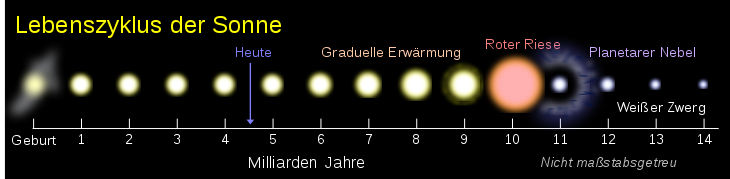
\includegraphics[width=\textwidth]{images/life_cycle_sun.png}
    \caption[Lebenszyklus der Sonne]{Lebenszyklus der
    Sonne\footnotemark}
    \label{img:life-cycle-sun}
  \end{figure}
  \footnotetext{https://de.wikipedia.org/wiki/Sonne}
\end{document}
